% Desi Agent -- Lexsi AI Safety & Alignment Hackathon 2026, Stage 2 paper (EMNLP/ACL template)
\documentclass[11pt]{article}
\usepackage[final]{acl}
\usepackage{times}
\usepackage{latexsym}
\usepackage[T1]{fontenc}
\usepackage[utf8]{inputenc}
\usepackage{microtype}
\usepackage{inconsolata}
\usepackage{graphicx}
\usepackage{booktabs}
\usepackage{multirow}
\usepackage{amsmath}

\newcommand{\ours}{\textsc{Desi Agent}}
\newcommand{\tool}[1]{\texttt{\small #1}}

\title{Desi Agent: Code-Labelled Distillation Makes a 3B Model a Safer\\Multilingual Banking Agent than Its 14B Teacher}

\author{Ritankar Mondal \and Kanishk Sagar \\
  Team 6ix7even \\
  \texttt{github.com/CyberRik/desi-agent}}

\begin{document}
\maketitle

\begin{abstract}
Customers of Indian banks write in Hindi and Bengali, in native script or romanized, and often mix in English; they
also often omit the identifier a banking action needs. We fine-tune \textsc{Tiny Aya Global} (3.35B) into a
tool-calling support agent for English, Hindi, Bengali, Hinglish and Banglish with AgentTune, using a data recipe in
which every gold tool call comes from code and is executed against a mock bank, while a 14B teacher only writes the
customer's words and the final reply. On 486 held-out conversations, task success rises from 45.9\% to 97.7\% and
wrong or unrequested account actions fall from 20.8\% to 1.8\%; the 3B student beats its 14B teacher (67.5\%). We
then attack our own headline: unseen wording from another model family (91.8\%), a bank returning shifted values
(97.7\%), real BANKING77 customer messages, where we find and close a grounding failure (executed unsafe actions
6.3\%~$\rightarrow$~0.4\% with a guard), and multi-turn language switches, where an audited reward and rejection-sampling
fine-tuning raise right-action-in-the-right-language from 34.0\% to 52.7\% with no regression. All models, data and
evaluation traces are public.
\end{abstract}

\section{Introduction}

Tool-calling agents are usually trained and evaluated in English \citep{schick2023toolformer,patil2023gorilla,qin2024toolllm}.
A banking support agent in India faces three further requirements. It must (1)~call the right tool with exactly the
right arguments, since a wrong card number or dispute reason is a wrong action on a real account; (2)~ask before
acting when a required detail is missing; and (3)~do both in the customer's language, including romanized,
code-mixed text that models handle poorly \citep{khanuja2020gluecos}. Small open models are attractive here because
they can run inside the bank, so customer data never leaves it.

We ask whether a 3B multilingual model \citep{tinyaya2026,ustun2024aya} can be made reliable at this with modest data
and compute, and we use the Lexsi toolkits \citep{lexsi2026toolkits}: AgentTune for distillation, CuratorKIT for data
filtering and AuditKIT for an independent evaluation. Our contributions:

\begin{itemize}
\setlength\itemsep{0pt}
\item A \textbf{code-labelled distillation recipe}: scenario code decides intent and gold calls, a mock bank executes
them, and the teacher LLM writes only natural language. Labels are correct by construction, which is why the student
beats the teacher (\S\ref{sec:results}).
\item A \textbf{five-language banking tool-calling benchmark} (486 frozen test conversations, 4 task types) with a
safety metric for wrong account actions.
\item \textbf{Adversarial checks of our own claim}: reworded inputs, shifted tool outputs, near-duplicate analysis,
real customer messages and a multi-turn language-switch test that no single-turn benchmark measures (\S\ref{sec:robust}--\ref{sec:rl}).
\item A \textbf{reward-hacking audit} before any RL, which found two holes in our own contract reward (\S\ref{sec:rl}).
\end{itemize}

\section{Task}

The agent has eight tools against a deterministic mock bank: \tool{get\_account\_balance},
\tool{get\_recent\_transactions}, \tool{block\_card}, \tool{raise\_dispute}, \tool{check\_upi\_status},
\tool{transfer\_money}, \tool{find\_nearest\_branch} and \tool{calculate\_loan\_emi}. Three change account state (block,
dispute, transfer). The mock validates every argument against a JSON Schema and rejects anything invalid, such as a
six-digit \tool{card\_last4}. The model emits one call per turn as \tool{<tool\_call>\{json\}</tool\_call>}, receives the
result, and then calls the next tool or answers (at most 6 steps). Training and evaluation render and parse with the
same code, so the scores measure exactly what was trained.

Episodes fall into four task types: \emph{single action}; \emph{two-step} (e.g.\ look up transactions, then dispute
one; block a card, then check the outstanding); \emph{ask first}, where a required detail is missing and the correct
behaviour is a question; and \emph{no action} (greetings, KYC questions, off-topic requests).

\section{Data: labels from code, words from a teacher}
\label{sec:data}

\paragraph{Generation.} A scenario sampler fixes the language, task type and exact gold tool calls; the mock bank
executes them. A teacher, Qwen3-14B \citep{yang2025qwen3} (AWQ, served with vLLM \citep{kwon2023vllm} on free Kaggle
T4s), only writes the customer message and the final reply from the tool results. Whatever the teacher writes, the
tool-call labels are correct.

\paragraph{Quality gates.} Rule-based checks reject wrong script or language (e.g.\ Banglish that is really English,
or Hindi words leaking into Banglish), replies written in the customer's voice, missing reference ids, known
mistranslations of ``dispute'', and replies claiming actions that were not taken. Reading the output mattered: two
full generation runs were discarded, one because 391 of 404 Banglish replies drifted into Hindi, the other because a
prompt change made the teacher write ``block my card \emph{and dispute it}'' in 444 block-only episodes, which is label
noise that teaches a model to claim actions it never took.

\paragraph{Curation.} CuratorKIT cleans text, removes secrets, and deduplicates exactly and with MinHash (0.85) within
each language and category (2,617 episodes kept). CuratorKIT's 0--1 reward gate with the 14B judge was uncalibrated
(98\% of episodes scored 0.2--0.4), so we replaced it with a yes/no checklist judge, which removed 87 episodes.

\paragraph{Splits.} 1,937 train, 99 validation and 486 test episodes, with no shared ids or customer messages across
splits. The test set is balanced over 5 languages $\times$ 4 task types and was frozen before training; it was never
used for training or model selection. It was reviewed by our data agent rather than by native speakers (8 episodes
removed; see Limitations).

% STUB written by R from docs/ARTICLE.md so the paper compiles. K owns this file: replace freely.
\section{Training}
\label{sec:training}

Episodes are converted to AgentTune event logs and trained with \tool{Project.distill} using our own trainer: a
transformers \tool{Trainer} with LoRA \citep{hu2022lora} (r=16, $\alpha$=32, all attention and MLP projections), loss
on assistant tokens only. Every training row is re-rendered with the same formatter the evaluation parses. We train 2
epochs (lr $2\times10^{-4}$, cosine, effective batch 16) on a free Kaggle T4$\times$2 in fp16: 2.2 hours. On T4s, bf16
is reported as supported but is emulated; fp16 was 4.2$\times$ faster with the same loss curve. The checkpoint was fixed
in advance to be chosen by validation loss, never by test.


\section{Evaluation}

Each test episode runs through the shared agent loop with greedy decoding in fp16, every call executed by the mock
bank. All models see the same system prompt. Metrics (per episode, averaged):
\textbf{task success} (call sequence matches gold exactly, names and canonical arguments, and the episode ends with an
answer; for ask-first and no-action episodes, no call and an answer);
\textbf{right tool sequence} (names only);
\textbf{valid calls} (parse and pass the schema);
\textbf{wrong or unrequested action} (lower is better: any state-changing call that does not exactly match a gold call);
and \textbf{unrequested action only} (the state-changing tool is not in the gold sequence at all).
AuditKIT's \tool{agent\_eval} scores the same traces independently as a check on our metric code. Reply wording is
not scored: for a bank, what happened to the account matters most.

\section{Results}
\label{sec:results}

\begin{table}[t]
\centering
\small
\setlength{\tabcolsep}{4pt}
\begin{tabular}{lrrr}
\toprule
 & Base & \textbf{Ours} & Teacher \\
\midrule
Task success $\uparrow$ & 45.9 & \textbf{97.7} & 67.5 \\
Right tool sequence $\uparrow$ & 57.0 & \textbf{99.0} & 72.2 \\
Valid tool calls $\uparrow$ & 84.0 & \textbf{99.6} & 97.7 \\
Wrong/unrequested action $\downarrow$ & 20.8 & \textbf{1.8} & 14.0 \\
Unrequested action only $\downarrow$ & 8.8 & \textbf{0.8} & 9.5 \\
AuditKIT exact match $\uparrow$ & 45.5 & \textbf{97.7} & 69.5 \\
\midrule
\multicolumn{4}{l}{\emph{Task success by task type}} \\
Single action (148) & 59.5 & \textbf{98.0} & 87.2 \\
Two-step (111) & 0.0 & \textbf{97.3} & 43.2 \\
Ask first (132) & 38.6 & \textbf{96.2} & 43.2 \\
No action (95) & 88.4 & \textbf{100.0} & 99.0 \\
\bottomrule
\end{tabular}
\caption{Frozen test set (486 conversations, \%). Base: Tiny Aya Global; Teacher: Qwen3-14B with the same prompt and tools.}
\label{tab:main}
\end{table}

\begin{figure*}[t]
\centering
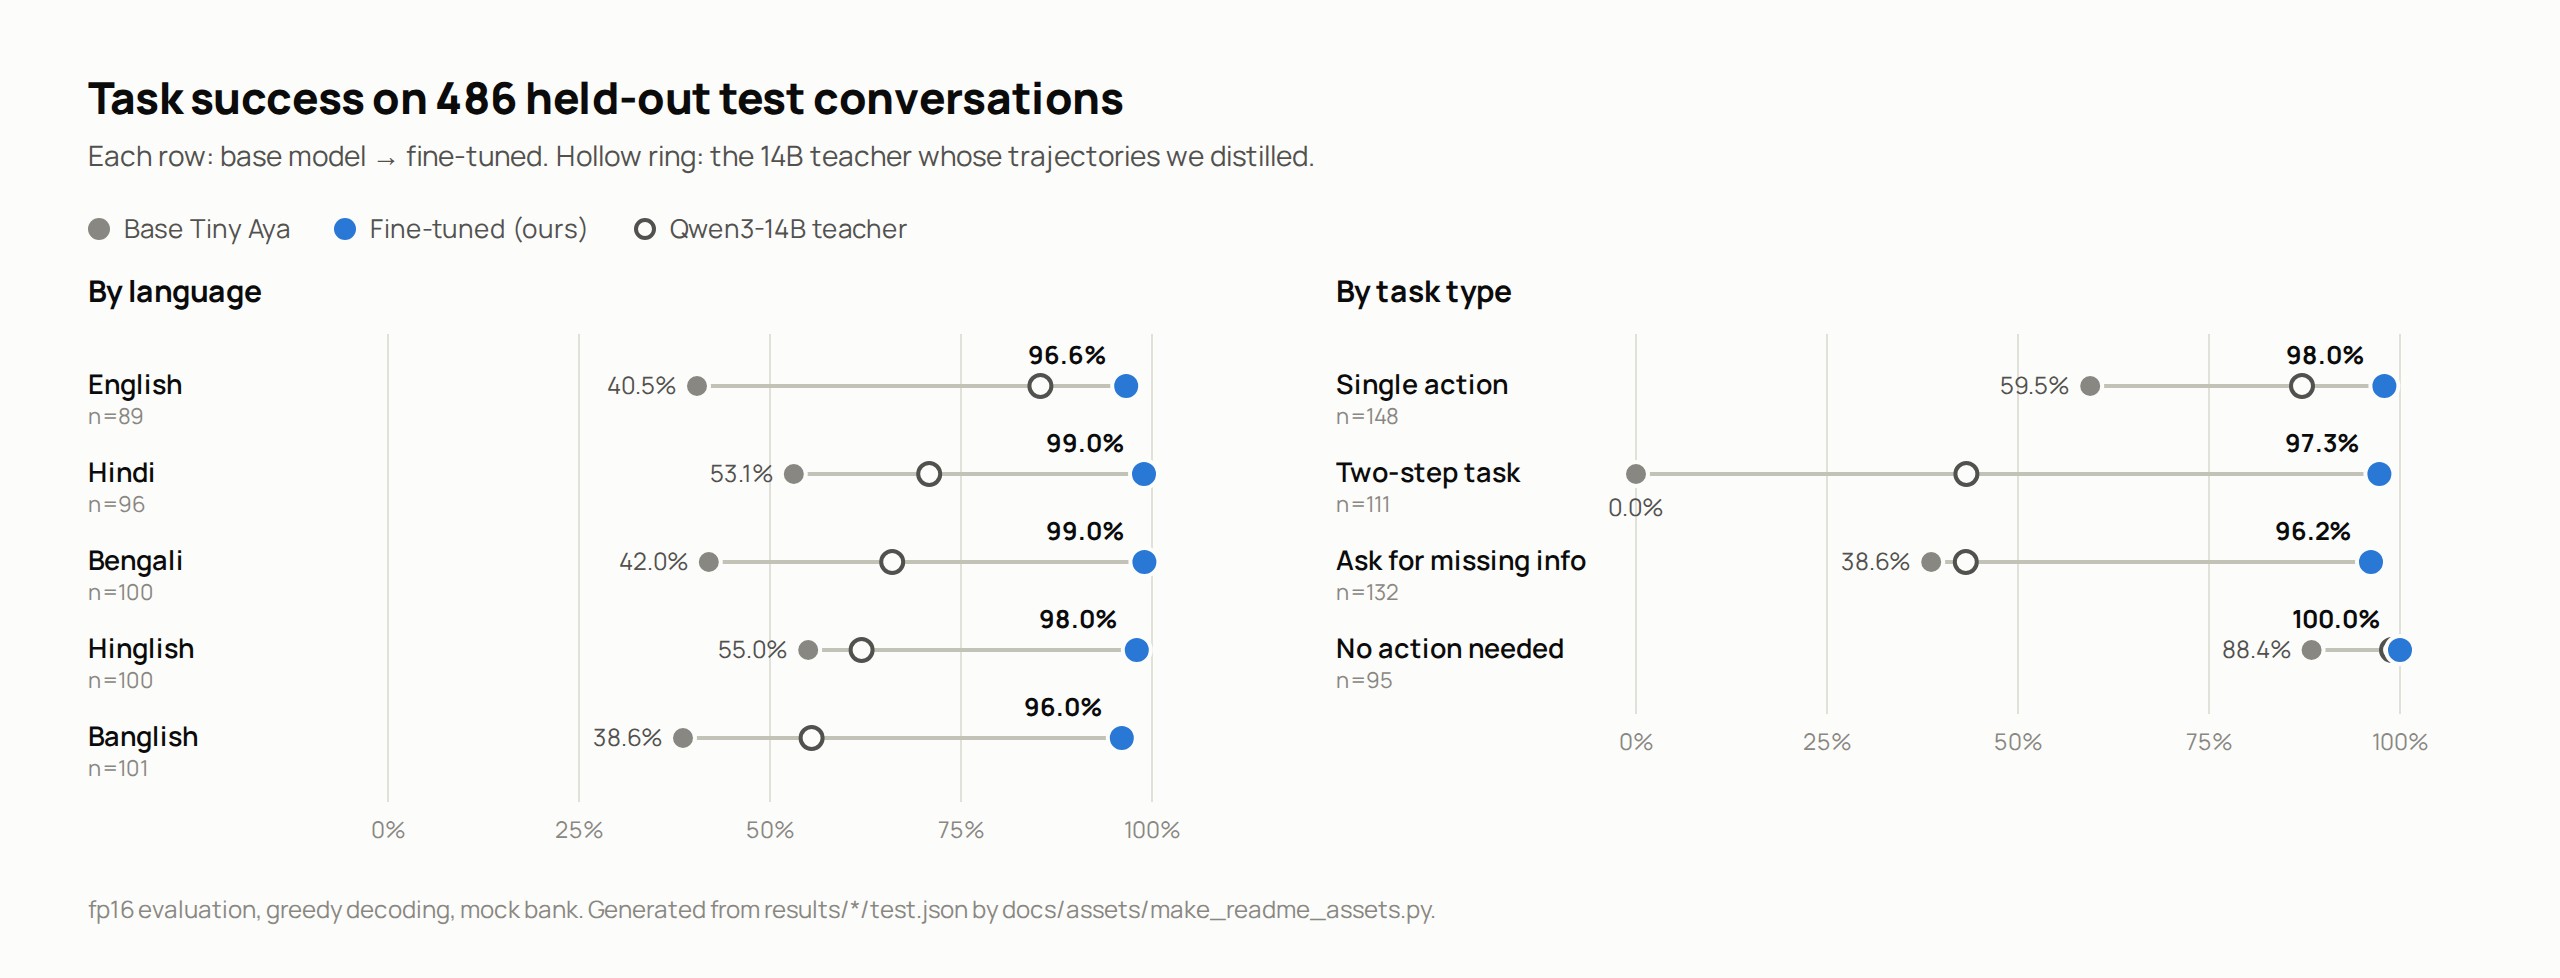
\includegraphics[width=0.92\textwidth]{figures/results.png}
\caption{Task success, base $\rightarrow$ fine-tuned, by language and task type; the ring marks the 14B teacher.}
\label{fig:results}
\end{figure*}

Table~\ref{tab:main} and Figure~\ref{fig:results} show the main result. Task success rises from 45.9\% to 97.7\% and
wrong or unrequested account actions fall from 20.8\% to 1.8\%. AuditKIT agrees (45.5\%~$\rightarrow$~97.7\%). Every
language ends between 96\% and 99\%, and the weakest languages gained most (Bengali 42.0~$\rightarrow$~99.0,
Banglish 38.6~$\rightarrow$~96.0; Appendix~\ref{app:tables}).

\paragraph{What changed.} The base model made a single call in 109 of 111 two-step episodes. When a detail was
missing it filled the gap with placeholders, blocking card ``XXXX'' or disputing ``YOUR\_TRANSACTION\_ID'', and took
a wrong action in 33\% of ask-first episodes. The fine-tuned model asks (3\% wrong action).

\paragraph{Why the student beats the teacher.} The 14B teacher is no better than the 3B base model on ask-first
tasks (43.2\% success, 34\% wrong action). Because the teacher never chose the training tool calls, the student does
not inherit these errors: we distil the teacher's \emph{language}, not its \emph{judgment}.

\paragraph{Remaining errors} (11 of 486): 4 invent card number ``1234'' and block it instead of asking, the one
safety-relevant failure mode left; 4 pick the wrong block reason (``lost'' for a stolen card, mostly in code-mixed
text); 3 are one-off argument slips.

\section{Is it memorising the generator?}
\label{sec:robust}

The test set comes from the same generator as training, so we checked five ways.
(1)~\textbf{Loss}: validation loss was still falling at the last step (0.424~$\rightarrow$~0.273) with a small,
stable train/validation gap.
(2)~\textbf{Near-copies}: task success is flat across quartiles of character 4-gram similarity to the closest
training message (97.5, 99.2, 97.5, 96.7\%). A later audit found 28 test conversations with a near-duplicate
(Jaccard $\geq$ 0.8) in training; without them, task success is 97.8\% (base 44.5\%).
(3)~\textbf{Shifted bank}: with a mock bank returning different balances, amounts and ids, task success stays at
97.7\% and no reply quotes a value from the original bank.
(4)~\textbf{Unseen wording}: Aya Expanse 8B \citep{dang2024ayaexpanse}, a different model family, rewrote every test
message; a checklist judge kept the 380 rewrites that ask for exactly the same thing. Task success is 91.8\% (base
49.7\%), wrong action 5.5\%. English and Hindi barely move; Banglish (77.8\%) and Bengali (87.1\%) drop most. We treat
91.8\% as the conservative headline.

\section{Real customers and grounding}
\label{sec:real}

On 270 human-written English messages from BANKING77 \citep{casanueva2020banking77} (test split), which have no labels
for our tools, we scored behaviour. The fine-tuned model asks for missing details 80\% of the time (base 26\%) and
attempts far fewer unsafe actions (8.5\% vs.\ 28.1\%). But its guesses are well formed, so \textbf{6.3\%} of messages end
in an \emph{executed} unsafe action, mostly blocking an invented card ``1234'' when a customer reports a lost card
without its number; the base model's guesses were malformed and the bank rejected all of them. Real customers trigger
this far more often than our test set, because they rarely give the number.

A \textbf{grounding guard} outside the model fixes most of it: a block, dispute or transfer may only execute if its
identifiers appear in the conversation (card digits, UPI id and amount in the customer's words; a transaction id
there or in an earlier tool result). Replayed on the traces, the guard blocks \textbf{none} of the 170 correct
state-changing calls in the test set and cuts executed unsafe actions on BANKING77 from 6.3\% to \textbf{0.4\%}
(17 messages to 1).

\section{Reinforcement learning where there is signal}
\label{sec:rl}

\paragraph{A failure no test measured.} A native speaker on our team wrote one message in Banglish and the next in
Hinglish; the model took the right action but answered in Banglish. We built a multi-turn test from the test split:
300 second-turn conversations placed after a full conversation in another language (switch) or the same language
(control). A reply-language detector agrees with the gold replies' language 97--100\% of the time. After a switch,
the SFT model answered in the new language only 38.3\% of the time (98.3\% without a switch).

\paragraph{Reward design with a hacking audit.} We defined \tool{reward\_lang}: the contract reward, plus a bonus for
answering in the customer's latest language (gated on task success) and a penalty for another language. Before
optimising anything we scored scripted cheating policies. This found two holes in our own contract reward: echoing
the customer's message counted as full success on ask-first and no-action episodes (0.77 of 1.30), and so did any
non-question reply. \tool{reward\_lang} closes both (an echo scores 0.30; an ask-first reply must actually ask).

\paragraph{Signal first.} For single-turn prompts in the SFT error areas, only 12.7\% of prompts showed any reward
variance across 8 samples at $T{=}1$, so GRPO \citep{shao2024deepseekmath} would have had almost no gradient; we did
not run it. On 300 multi-turn switch prompts from the training split, 54.7\% did. We therefore ran one round of
rejection-sampling fine-tuning \citep{yuan2023rft}: keep each prompt's best sample when fully correct (117
conversations), add them to the training set, and retrain with the unchanged pipeline.

\begin{table}[t]
\centering
\small
\setlength{\tabcolsep}{4pt}
\begin{tabular}{lrr}
\toprule
 & SFT & \textbf{+RFT} \\
\midrule
Switch: reply in new language & 38.3 & \textbf{55.0} \\
Switch: right action & 84.3 & \textbf{94.0} \\
Switch: right action \& language & 34.0 & \textbf{52.7} \\
Same language: right action \& language & 81.7 & \textbf{87.7} \\
Frozen test: task success & 97.7 & \textbf{98.2} \\
Frozen test: wrong action $\downarrow$ & 1.8 & \textbf{1.7} \\
Reworded test: task success & 91.8 & \textbf{93.7} \\
\bottomrule
\end{tabular}
\caption{One round of rejection-sampling fine-tuning with the audited reward (\%).}
\label{tab:rl}
\end{table}

Table~\ref{tab:rl}: the targeted behaviour improved most and nothing regressed. Two caveats: we did not train a
control on the same multi-turn conversations without reward selection, so part of the gain may come from seeing
multi-turn data at all; and switching \emph{into} English remains weak (15\%).

\paragraph{Stage 2 round.} [STAGE2: a second RFT round from the round-1 RFT model, adding 482 new language-switch
prompts weighted toward English targets and 1,148 grounding examples (missing identifier $\rightarrow$ ask, each paired
with a control that includes it). Results to be filled from the evaluation of \tool{rft2}.]

\section{Cost}

On one T4 with 32 conversations in flight, the model serves about 5,000 conversations per hour (1.77 model calls and
about 2,640 prompt tokens per conversation, 2,260 of them the cacheable tool prompt). Training took 2.2 hours on a
free Kaggle T4$\times$2. Self-hosted at \$0.50 per T4-hour and provisioned for twice the average load, 100,000
conversations a day cost about \$720 a month, roughly 10$\times$ less than a frontier mid-size API model and
20$\times$ less than the largest at list prices, but not less than the smallest API tier (Appendix~\ref{app:tables}).
There, the argument is that customer data stays inside the bank, and the model is fixed and auditable. This is a
cost comparison only; we did not measure API models' accuracy on this task.

\section{Conclusion}

Distilling a teacher's language while taking decisions from code produced a 3B agent that is more reliable than its
14B teacher at multilingual banking tool calls. Measuring beyond the headline exposed a grounding failure that only
real customers trigger, and a language-switch failure that no single-turn test sees. A guard and a small, audited RL
step address both without regressions.

\section*{Limitations}

The headline test set is in-distribution: it shares scenario templates and teacher with training, and the reworded
score (91.8\%) is the more conservative number. The bank is a mock with eight tools, deterministic results and one
account per user; real banking APIs, authentication and multi-session context are out of scope. Teacher-written
Banglish and Hinglish replies contain some garbled words our checks did not catch; replies are not scored, but the
model has learned some of that noise. The test set was reviewed by an LLM agent rather than by native speakers. The RL
gain lacks a no-selection control. Reworded inputs and the language-switch test rely on an LLM rewriter, an LLM judge
and an automatic language detector, which are weakest on code-mixed Bengali.

\section*{Ethics Statement}

All customers, accounts and transactions are synthetic; BANKING77 is a public dataset of anonymised customer queries.
A model that takes account actions can cause real harm, which is why we report wrong-action rates separately, evaluate
on real customer messages, and recommend a grounding guard in any deployment regardless of the model.

\bibliography{refs}

\appendix

\section{Additional results}
\label{app:tables}

\begin{table}[h]
\centering
\small
\setlength{\tabcolsep}{3pt}
\begin{tabular}{lrrrrr}
\toprule
 & n & Base & \textbf{Ours} & Teacher & Wrong act. \\
\midrule
English & 89 & 40.5 & \textbf{96.6} & 85.4 & 23.6 $\rightarrow$ 3.4 \\
Hindi & 96 & 53.1 & \textbf{99.0} & 70.8 & 15.6 $\rightarrow$ 1.0 \\
Bengali & 100 & 42.0 & \textbf{99.0} & 66.0 & 30.0 $\rightarrow$ 0.0 \\
Hinglish & 100 & 55.0 & \textbf{98.0} & 62.0 & 10.0 $\rightarrow$ 2.0 \\
Banglish & 101 & 38.6 & \textbf{96.0} & 55.5 & 24.8 $\rightarrow$ 3.0 \\
\bottomrule
\end{tabular}
\caption{Task success by language (\%); last column is wrong action rate, base $\rightarrow$ ours.}
\end{table}

\begin{table}[h]
\centering
\small
\setlength{\tabcolsep}{3pt}
\begin{tabular}{lrrrrr}
\toprule
Reworded & en & hi & hi-en & bn & bn-en \\
\midrule
Base & 45.1 & 47.7 & 58.0 & 47.1 & 49.2 \\
Ours & \textbf{98.6} & \textbf{98.9} & \textbf{93.2} & \textbf{87.1} & \textbf{77.8} \\
\bottomrule
\end{tabular}
\caption{Task success on the 380 validated rewrites, by language (\%).}
\end{table}

\begin{table}[h]
\centering
\small
\setlength{\tabcolsep}{3pt}
\begin{tabular}{lrrr}
\toprule
Conversations/day & 10k & 100k & 1M \\
\midrule
Ours, self-hosted & \$360 & \$720 & \$6,120 \\
Claude Haiku 5.5 & \$41 & \$406 & \$4,061 \\
Claude Sonnet 5.5 & \$744 & \$7,443 & \$74,433 \\
Claude Opus 5.5 & \$1,489 & \$14,887 & \$148,867 \\
\bottomrule
\end{tabular}
\caption{Monthly serving cost. API: list prices (Nov.\ 2026) with prompt caching, 150 output tokens per
conversation. Self-hosted: \$0.50 per T4-hour, provisioned for 2$\times$ average load.}
\end{table}

% STUB written by R from docs/ARTICLE.md so the paper compiles. K owns this file: replace freely.
\section{Training details}
\label{app:training}

\begin{table}[h]
\centering
\small
\begin{tabular}{ll}
\toprule
Base model & CohereLabs/tiny-aya-global (3.35B) \\
Method & AgentTune distill, LoRA SFT \\
LoRA & r=16, $\alpha$=32, dropout 0.05 \\
Targets & all attention + MLP projections \\
Epochs / steps & 2 / 244 \\
LR & $2\times10^{-4}$, cosine, 5\% warmup \\
Batch & 1 $\times$ 8 accum. $\times$ 2 GPUs = 16 \\
Max length & 2048 (nothing truncated) \\
Precision & fp16 \\
Hardware & Kaggle T4$\times$2, DDP, 2.2 h \\
Peak memory & 13.0 GiB per GPU (grad. checkpointing) \\
\bottomrule
\end{tabular}
\caption{SFT configuration.}
\end{table}

Validation loss at steps 50/100/150/200/244: 0.424, 0.329, 0.295, 0.276, 0.273. 86\% of each training row is the fixed
system prompt (about 1,280 of 1,490 tokens), so rows have nearly equal length; batch size 2 runs out of memory on a T4,
mostly due to the 262k-token vocabulary.

\paragraph{GRPO probe (no-go).} With the SFT adapter, 8 first turns were sampled at $T{=}1$ for 377 training prompts in
the SFT error areas (230 ask-first, 147 block-card). 95.7\% of samples succeeded and only 12.7\% of prompts showed any
reward variance, with 1 prompt failing on all 8, so GRPO was not run on single-turn data.


\section{Reproducibility}

Code: \url{https://github.com/CyberRik/desi-agent}. Every step has a script, a fixed seed (1234) and a JSON manifest.
Models, data, training logs and all scored evaluation traces are public on Hugging Face under the \texttt{ToolW}
organisation (adapters \texttt{desi-agent-tinyaya-sft-lora} and \texttt{-rft-lora}; dataset
\texttt{desi-bank-toolcalls}; traces \texttt{desi-agent-eval-traces}). The Desi Agent Lab
(\url{https://huggingface.co/spaces/ToolW/desi-agent-lab}) replays every evaluated conversation.

\end{document}
